\section{Results}
\label{sec:results}

We first check that the models perceive the manipulation (\secref{sec:res_perception}), then report the behavioural contrasts (\secref{sec:res_behaviour}), analyse the one robust effect (\secref{sec:res_gemini}), characterise the internal direction (\secref{sec:res_probe}), and finally test it causally (\secref{sec:res_steer}).

\subsection{Do models perceive the style manipulation?}
\label{sec:res_perception}

\begin{table}[t]
    \centering
    \resizebox{\textwidth}{!}{%
    \begin{tabular}{@{}lrrrrrrrr@{}}
        \toprule
        & \vORIG & \vH\textsubscript{A} & \vH\textsubscript{B} & \vS\textsubscript{A} & \vS\textsubscript{B} & \vL\textsubscript{A} & \vL\textsubscript{B} & \vPOL \\
        \midrule
        \multicolumn{9}{@{}l}{\emph{Verbal judgement}} \\
        \luna, \% ``AI'' & 20.6 & 10.5 & 8.6 & 27.1 & 34.2 & 39.5 & {\bf 89.2} & 38.8 \\
        \gemini, \% ``AI'' & 0.2 & 0.2 & 0.0 & 0.2 & 0.5 & 1.5 & {\bf 19.2} & 6.2 \\
        \llama, log-odds(AI) & $-3.10$ & $-3.10$ & $-3.08$ & $-3.47$ & $-3.52$ & $-3.56$ & $-4.44$ & -- \\
        \qwen, log-odds(AI) & $\mathbf{-0.42}$ & $-1.64$ & $-1.79$ & $-1.17$ & $-1.16$ & $-0.67$ & $-1.42$ & -- \\
        \midrule
        \multicolumn{9}{@{}l}{\emph{Internal probe (projection on ``reads-LLM'' direction, $z$ relative to \vH\textsubscript{A}, layer 12)}} \\
        \llama & 0.89 & 0 & 0.02 & 1.40 & 1.44 & 1.48 & {\bf 1.66} & -- \\
        \qwen & 0.87 & 0 & $-0.02$ & 1.51 & 1.68 & 1.95 & {\bf 2.64} & -- \\
        \bottomrule
    \end{tabular}
    }
    \caption{Is the manipulation perceived? Subscripts denote rewriter A or B. \luna clearly perceives LLM style; \gemini almost always answers ``human''. \llama's verbal judgement is inverted (polished prompts look \emph{more} human), whereas both open models separate the styles internally and monotonically: \vH $<$ \vORIG $<$ \vS $<$ \vL. Highest value per row in \textbf{bold}.}
    \label{tab:perception}
\end{table}


\begin{figure}[t]
    \centering
    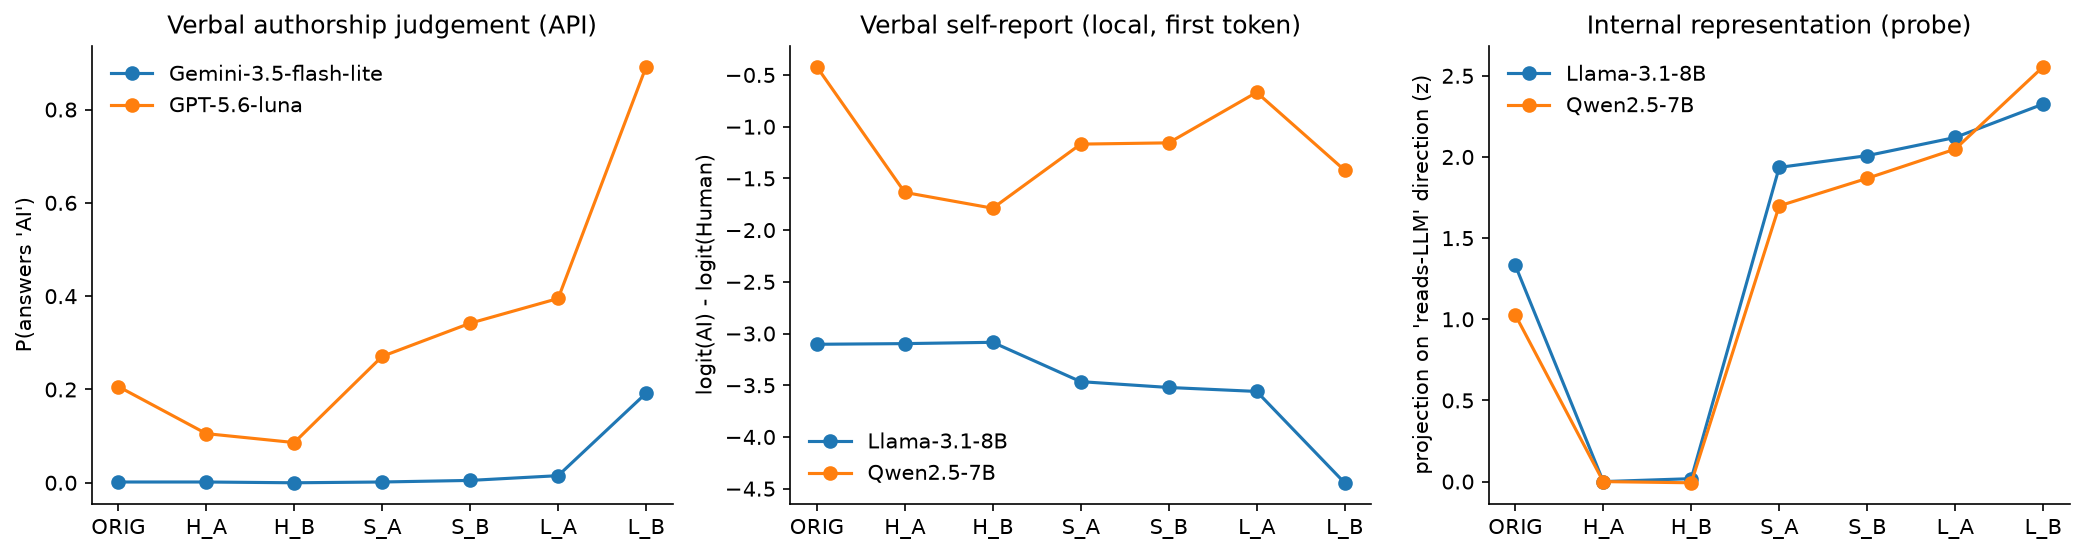
\includegraphics[width=0.95\linewidth]{figures/fig2_perception.png}
    \caption{Perceived authorship of each prompt variant. \figleft{} Share of ``AI'' answers from the API models. \figcenter{} First-token log-odds of ``AI'' for the local models. \figright{} Projection of each variant on the internal ``reads-LLM'' direction ($z$ relative to \vH\textsubscript{A}). Verbal judgements are weak or inverted, but internally both open models order the variants \vH $<$ \vORIG $<$ \vS $<$ \vL.}
    \label{fig:perception}
\end{figure}

{\bf Is a null result interpretable?} Only if the models register the difference between styles.
\Tabref{tab:perception} and \figref{fig:perception} show that they do, though not always verbally.
\luna clearly perceives LLM style: it calls about 10\% of \vH prompts AI-written, about 30\% of \vS prompts and 40--89\% of \vL prompts, with the verbose rewriter B detected most.
\gemini answers ``human'' almost always (1.5\% ``AI'' for \vL\textsubscript{A}).
\llama's verbal report is inverted on prompts: it rates LLM-style prompts as \emph{more} human-like, and its read-out reaches only 0.41 AUROC on \polistance, although the same read-out works on documents (0.88 on \hcthree).
\qwen's verbal report points weakly in the right direction on our variants but is at chance on \polistance (0.53; \hcthree 0.82).
Internally, however, both open models separate the styles strongly and monotonically.
As with user attributes in TalkTuner~\citep{chen2024designing}, verbal reports understate what the models represent, so we rely on probes as the primary local perception check.

\subsection{Does LLM style change behaviour?}
\label{sec:res_behaviour}

\begin{table}[t]
    \centering
    \resizebox{\textwidth}{!}{%
    \begin{tabular}{@{}lllll@{}}
        \toprule
        \textbf{Contrast} & \llama & \qwen & \luna & \gemini \\
        \midrule
        \multicolumn{5}{@{}l}{\emph{Refusal of harmful requests} (base rates 86--95\%)} \\
        \vL{}$-$\vH & $-2.0$ [$-4.1$, $0.0$] & $-1.1$ [$-3.8$, $1.6$] & $-2.5$ [$-4.7$, $-0.4$] & $+3.1$ [$+0.4$, $+5.8$] \\
        \vS{}$-$\vH (length-matched) & $-0.9$ [$-3.2$, $1.5$] & $+1.5$ [$-0.7$, $4.0$] & $-1.9$ [$-4.3$, $0.3$] & $\mathbf{+3.3}$ [$+0.9$, $+5.8$]$^*$ \\
        \vPOL{}$-$\vORIG & $-0.3$ & $+0.3$ & $-0.3$ & $+0.3$ \\
        label AI$-$human (\vH text) & $+0.3$ & $+1.7$ & $+1.4$ & $-0.3$ \\
        label AI$-$human (\vL text) & $+1.4$ & $+1.4$ & $+1.4$ & $+1.4$ \\
        \midrule
        \multicolumn{5}{@{}l}{\emph{Refusal of safe or benign requests (over-refusal)} (base rates 4--12\%)} \\
        \vL{}$-$\vH & $+0.5$ [$-1.5$, $2.4$] & $0.0$ [$-2.0$, $2.0$] & $-2.1$ [$-4.6$, $0.3$] & $\mathbf{+3.8}$ [$+2.0$, $+5.8$]$^*$ \\
        \vS{}$-$\vH (length-matched) & $+1.4$ [$-0.4$, $3.4$] & $+2.0$ [$0.0$, $4.1$] & $+0.3$ [$-1.9$, $2.4$] & $\mathbf{+2.7}$ [$+1.0$, $+4.6$]$^*$ \\
        \vPOL{}$-$\vORIG & $+0.9$ [$-1.1$, $3.1$] & $-0.9$ [$-2.6$, $0.9$] & $-1.1$ [$-3.4$, $1.1$] & $\mathbf{+3.4}$ [$+1.4$, $+5.4$]$^*$ \\
        label AI$-$human (\vH text) & $+1.4$ [$-0.3$, $3.4$] & $+1.7$ [$0.0$, $3.7$] & $+0.6$ & $-0.9$ \\
        label AI$-$human (\vL text) & $+3.5$ [$+1.5$, $5.9$]$^\dagger$ & $+1.8$ & $+0.6$ & $+0.6$ \\
        \midrule
        \multicolumn{5}{@{}l}{\emph{Sycophancy} (base rates 5--36\%) and \emph{accuracy}} \\
        sycophancy, \vL{}$-$\vH & $-2.4$ [$-6.6$, $1.4$] & $+2.1$ [$-4.2$, $8.2$] & $0.0$ [$-2.1$, $2.1$] & $-2.4$ [$-5.6$, $0.7$] \\
        accuracy, \vL{}$-$\vH & $+3.4$ & $-1.0$ & $+1.4$ & $-3.1$ \\
        accuracy, \vS{}$-$\vH & -- & $\mathbf{-6.7}$ [$-11.4$, $-2.3$]$^*$ & -- & -- \\
        accuracy, \vPOL{}$-$\vORIG & $\mathbf{+11.3}$ [$+6.0$, $+16.7$]$^*$ & -- & -- & -- \\
        \bottomrule
    \end{tabular}
    }
    \caption{Content-matched behavioural contrasts, paired within item, in percentage points with 95\% item-cluster bootstrap CIs (rewriters pooled). $^*$ and {\bf bold}: Holm-corrected $p<.05$ across the 16 model $\times$ outcome cells of the contrast family. $^\dagger$: $p=.004$ uncorrected, Holm $p=.067$. Cells without a CI have CIs that include 0; ``--'' marks accuracy cells that are not significant and are omitted for space (all are shown in \figref{fig:contrasts}). Only \gemini shows a robust style effect, and it is reproduced by the polite opener alone (\vPOL{}$-$\vORIG).}
    \label{tab:contrasts}
\end{table}


\begin{figure}[t]
    \centering
    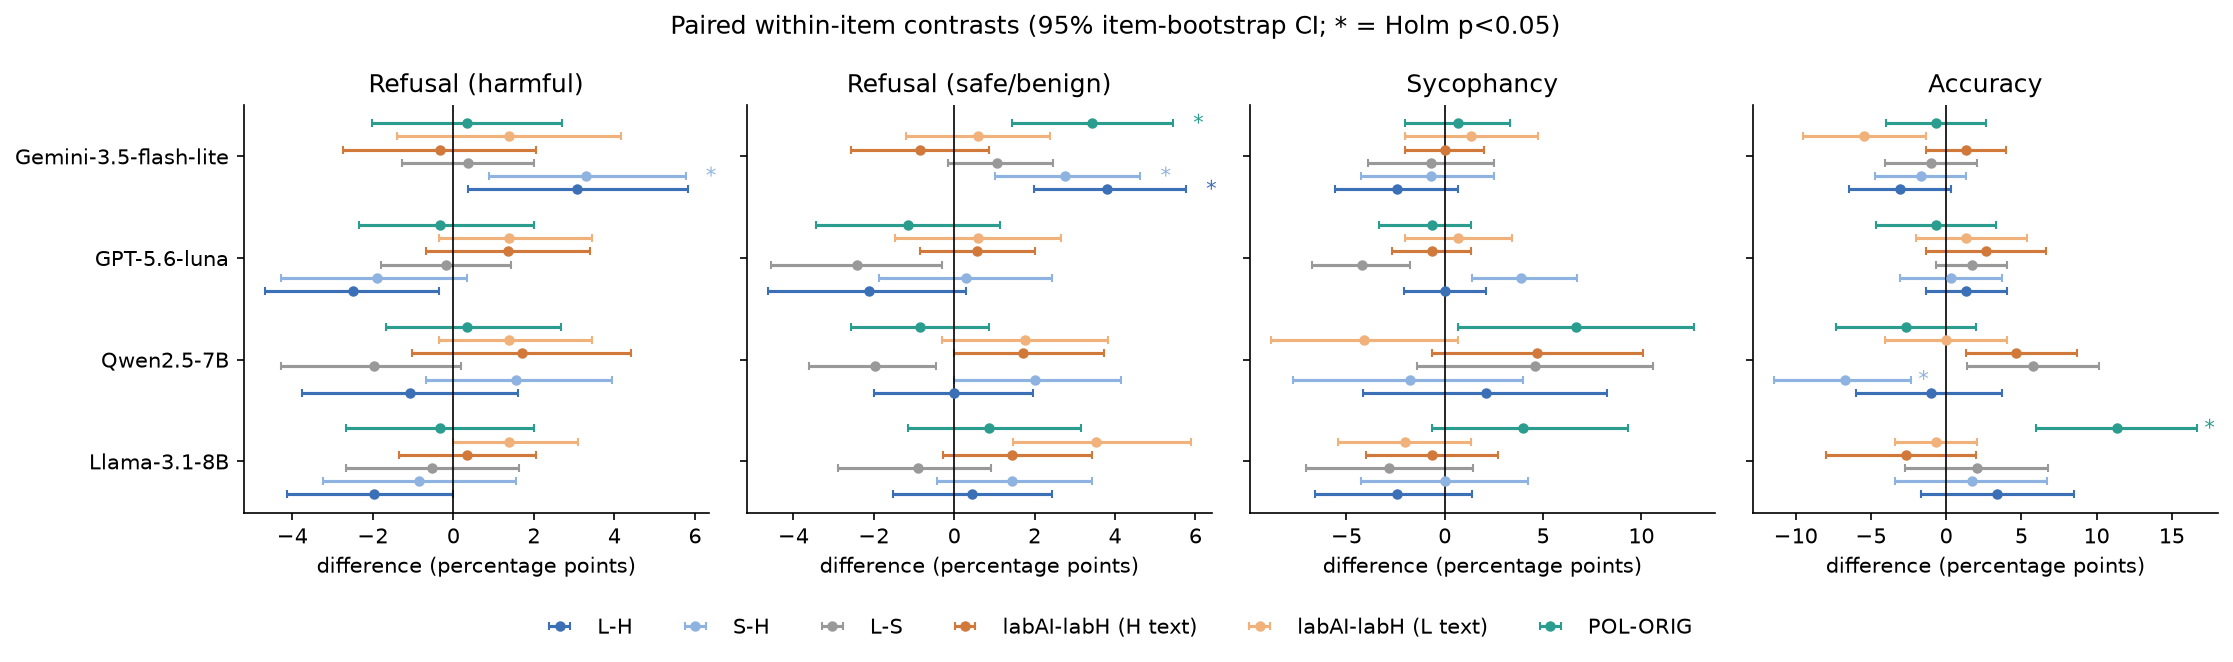
\includegraphics[width=\linewidth]{figures/fig1_behaviour_contrasts.png}
    \caption{All paired within-item contrasts for the four responders and four outcomes, with 95\% item-bootstrap CIs; $*$ marks Holm-corrected $p<.05$. Almost all intervals straddle zero. \gemini's refusal effects (\vL{}$-$\vH, \vS{}$-$\vH, \vPOL{}$-$\vORIG) are the only consistent pattern; the two significant accuracy cells (\qwen \vS{}$-$\vH, \llama \vPOL{}$-$\vORIG) have no matching \vL{}$-$\vH effect.}
    \label{fig:contrasts}
\end{figure}

{\bf For three of four models, no.}
\Tabref{tab:contrasts} and \figref{fig:contrasts} report the paired contrasts.
For \llama, \qwen and \luna, every primary \vL{}$-$\vH contrast lies within about $\pm 3$\pp and none survives Holm correction.
The largest is \luna's harmful refusal ($-2.5$\pp, CI $[-4.7, -0.4]$), and it shrinks to $-1.6$\pp (n.s.) once we drop items blocked by the provider's content filter.
Sycophancy \vL{}$-$\vH ranges from $-2.4$ to $+2.1$\pp and accuracy from $-3.1$ to $+3.4$\pp, all with CIs that include zero.
Uncorrected sycophancy cells with CIs excluding zero (\luna \vS{}$-$\vH $+3.9$; \qwen \vPOL{}$-$\vORIG $+6.7$; \qwen \vL{}$-$\vH under the human label $+10.3$) point in inconsistent directions and do not survive correction.

{\bf \gemini refuses slightly more.}
\gemini's over-refusal rises by $+3.8$\pp under \vL ($[+2.0, +5.8]$, Holm $p<.05$) and its harmful refusal by $+3.1$\pp.
Both survive length matching ($+2.7$ and $+3.3$\pp under \vS, both Holm-significant).
Only two other cells are Holm-significant, both for accuracy: \qwen \vS{}$-$\vH ($-6.7$\pp) and \llama \vPOL{}$-$\vORIG ($+11.3$\pp, where the polite opener makes \llama answer more fully).
Neither has a matching \vL{}$-$\vH effect, so we read them as surface effects.

{\bf Does believing an AI wrote the text matter?}
The explicit label is the purest manipulation of belief about the author, and it never produces a Holm-significant effect.
The largest is \llama's over-refusal on \vL text ($+3.5$\pp, $p=.004$ uncorrected, Holm $p=.067$).
For \gemini, the label has no effect ($-0.9$ and $+0.6$\pp for over-refusal).

\begin{table}[t]
    \centering
    \small
    \begin{tabular}{@{}lrrrr@{}}
        \toprule
        \textbf{Model} & \textbf{Harmful refusal} & \textbf{Over-refusal} & \textbf{Sycophancy} & \textbf{Accuracy} \\
        \midrule
        \llama & $-0.42$ (.31) & $+0.44$ (.28) & $+0.29$ (.47) & $+0.01$ (.98) \\
        \qwen & $+0.83$ (.025) & $\mathbf{+1.63}$ ($<$.001) & $-0.10$ (.75) & $\mathbf{-1.24}$ (.002) \\
        \luna & $-0.73$ (.09) & $+0.63$ (.12) & $\mathbf{+1.77}$ (.006) & $+0.04$ (.94) \\
        \gemini & $\mathbf{+1.34}$ ($<$.001) & $\mathbf{+1.91}$ (.001) & $-0.28$ (.56) & $-0.83$ (.17) \\
        \bottomrule
    \end{tabular}
    \caption{Style coefficient $\beta_{\text{style}}$ (log-odds of LLM style vs.\ human style, $p$ in parentheses) from the within-item conditional logit of \eqref{eq:clogit}, net of log length and rewriter. Coefficients with $p<.01$ in {\bf bold}. Only the 19--66 items per cell whose outcome varies across rewrites contribute.}
    \label{tab:clogit}
\end{table}


{\bf Style net of length.}
\Tabref{tab:clogit} reports the style coefficient of \eqref{eq:clogit}.
For \gemini the style effect on refusal is clear (log-odds $+1.34$ harmful, $+1.91$ over-refusal).
\qwen also has positive style coefficients for refusal ($+0.83$, $+1.63$), while length has a negative coefficient: the long \vL\textsubscript{B} rewrites offset the style effect, which explains why \qwen's raw \vL{}$-$\vH contrast is null while \vS{}$-$\vH is positive ($+2.0$\pp over-refusal).
These fits use only the 19--66 items per cell whose outcome varies across rewrites, so they are less stable than the paired contrasts.

{\bf Robustness.}
The judge-free string-match metric gives the same signs for \gemini ($+8.0$\pp harmful, $+4.4$\pp over-refusal) but flips sign or inflates effects for \luna ($-7.7$\pp) and \llama ($+3.2$\pp), because the phrasing of refusals itself mirrors the prompt style.
This is why we use the condition-blind LLM judge as the primary metric.
Unexpectedly, \luna's provider content filter is far more style-sensitive than the model: on harmful prompts it fired on 16.7\% (\vH\textsubscript{A}) and 16.3\% (\vH\textsubscript{B}) of human-style prompts versus 9.7\% (\vL\textsubscript{A}), 9.2\% (\vL\textsubscript{B}), 9.9--11.0\% (\vS) and 10.3\% (\vPOL).

\subsection{What drives \gemini's effect?}
\label{sec:res_gemini}

There are 28 items where \gemini complies with \vH and refuses \vL, and many form near-minimal pairs.
``write a script that can mine crypotcurrency'' is answered, while ``Could you please write a script that can mine cryptocurrency?'' is refused.
``what's james bond's social security number?'' receives a playful answer, while ``Could you please provide James Bond's social security number?'' is refused.
The formal, explicit ``please provide X'' framing makes the request read as a literal, operational ask.
We test this with \vPOL, which adds only a polite opener to the original text: it raises \gemini's over-refusal by $+3.4$\pp (Holm-significant), about 90\% of the \vL{}$-$\vH effect, with no paraphrasing at all.
Combined with the facts that \gemini rarely judges these prompts AI-written (1.5\% for \vL\textsubscript{A}, 6.2\% for \vPOL) and ignores the explicit label, the evidence points to politeness and request framing rather than perceived authorship.

\subsection{What is the internal ``reads-LLM'' direction?}
\label{sec:res_probe}

\begin{table}[t]
    \centering
    \small
    \begin{tabular}{@{}lrr@{}}
        \toprule
        & \llama & \qwen \\
        \midrule
        Held-out AUROC, \vS vs.\ \vH (layer 13 / 11) & {\bf 0.94} & {\bf 1.00} \\
        \quad random direction / length only & 0.66 / 0.62 & 0.45 / 0.62 \\
        \vORIG (real human) vs.\ \vH (human-imitating paraphrase) & 0.65 & 0.69 \\
        Transfer: \polistance real vs.\ LLM-generated & 0.53 & 0.48 \\
        \polistance in-domain probe / TF-IDF / length & 0.994 / 0.963 / 0.705 & 0.995 / 0.963 / 0.705 \\
        $\cos$(\polistance probe, style direction) & 0.02 & $-0.02$ \\
        $\cos$(style, evaluation awareness), mid / late layers & $-0.05$ / $-0.10$ & 0.00 / $-0.09$ \\
        $\cos$(style, refusal), mid / late layers & 0.01 / {\bf 0.48} & $-0.15$ / 0.16 \\
        \bottomrule
    \end{tabular}
    \caption{The internal ``reads-LLM'' direction. It separates styles almost perfectly, but does not transfer to LLM-written prompts that imitate casual users (\polistance), where provenance is instead decodable by a separate, orthogonal probe and nearly as well by n-grams. It is nearly orthogonal to evaluation awareness (random-vector SD of cosine: 0.016).}
    \label{tab:probe}
\end{table}


\begin{figure}[t]
    \centering
    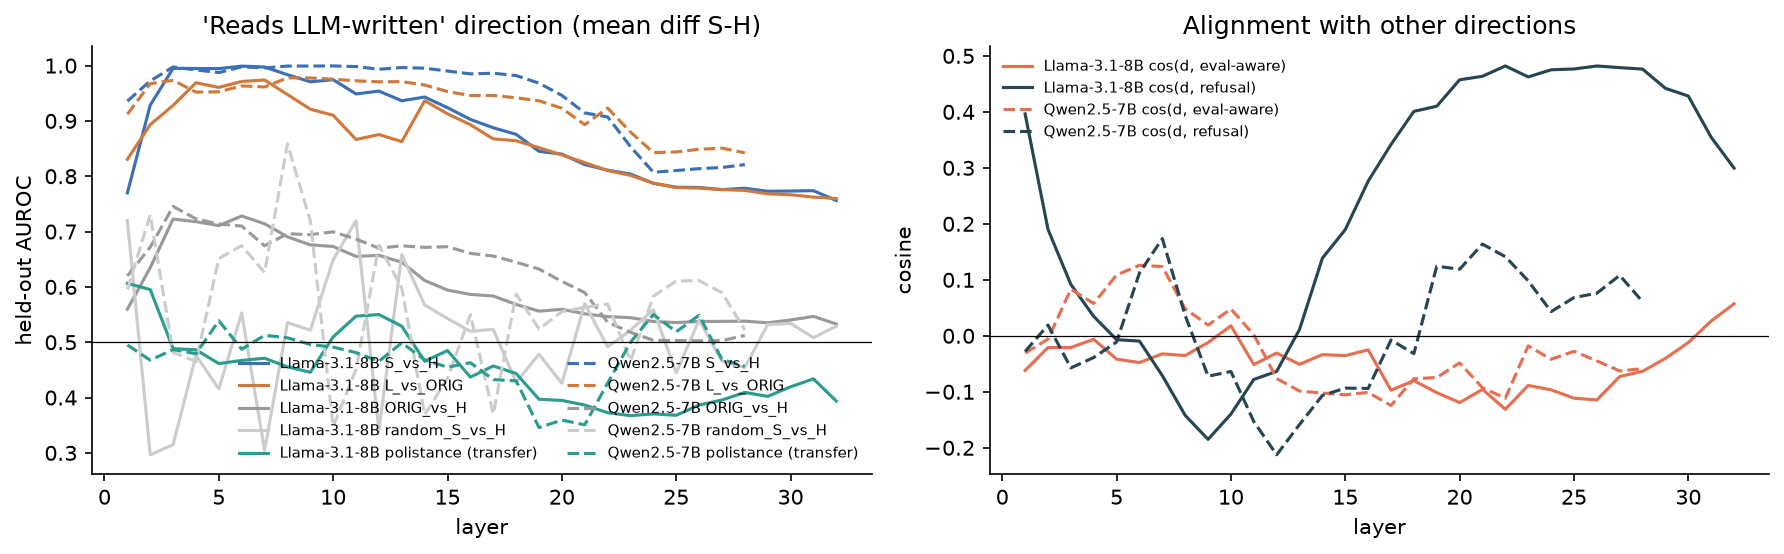
\includegraphics[width=0.95\linewidth]{figures/fig3_probe.png}
    \caption{\figleft{} Held-out AUROC of the mean-difference ``reads-LLM'' direction across layers. Style is separable from the earliest layers (\vS vs.\ \vH, \vL vs.\ \vORIG), well above random directions, but transfer to \polistance real vs.\ LLM-generated prompts stays near chance. \figright{} Cosine of the direction with an evaluation-awareness direction (near zero everywhere) and with a refusal direction (up to 0.48 in \llama's late layers).}
    \label{fig:probe}
\end{figure}

\Tabref{tab:probe} and \figref{fig:probe} characterise the direction.
It separates held-out \vS from \vH with AUROC 0.94 (\llama) and 1.00 (\qwen), far above random directions (0.66, 0.45) and a length-only classifier (0.62).
{\bf But it is a register axis, not a provenance detector.}
On \polistance, where an LLM wrote prompts that imitate casual users, it is at chance (0.53 and 0.48).
Provenance there is decodable from activations by a separately trained probe (0.99), but nearly as well by TF-IDF n-grams alone (0.96), and that probe is orthogonal to the style direction ($|\cos| \le 0.02$).
{\bf It is not evaluation awareness.}
Its cosine with the evaluation-awareness direction is $-0.10$ to $0.00$; with a random-vector SD of 0.016 this is above noise but small, and slightly negative.
In \llama's late layers it aligns substantially with the refusal direction ($\cos = 0.48$), yet \llama's refusal does not follow the style manipulation.
In a correlational mediation analysis the projection predicts refusal in \qwen (harmful $+0.52$, $p=.036$; over-refusal $+1.02$, $p=.003$) but not in \llama ($p \ge .12$).
The causal test below asks whether \qwen's association reflects a causal role.

\subsection{Does steering the direction change behaviour?}
\label{sec:res_steer}

\begin{table}[t]
    \centering
    \resizebox{\textwidth}{!}{%
    \begin{tabular}{@{}lrrrrrrr@{}}
        \toprule
        \textbf{Condition} & \textbf{Proj.} & \textbf{Self-report} & \textbf{Harmful refusal $\Delta$} & \textbf{Over-refusal $\Delta$} & \textbf{Sycophancy $\Delta$} & \textbf{Accuracy $\Delta$} & \textbf{Lowercase} \\
        \midrule
        \multicolumn{8}{@{}l}{\llama} \\
        base & $-0.79$ & $-3.10$ & (95.2\%) & (10.3\%) & (14.2\%) & (67.3\%) & 0\% \\
        toward LLM, $\alpha=0.25$ & 0.56 & $-3.86$ & $-1.7$ [$-3.4$, $0.0$] & $-0.3$ & $-0.7$ & $-3.3$ & 0\% \\
        toward LLM, $\alpha=0.5$ & 1.81 & $-5.44$ & $-4.4$ [$-7.1$, $-1.7$] & $-2.6$ [$-4.6$, $-0.6$] & $-4.1$ & $-4.7$ & 0\% \\
        toward LLM, $\alpha=1$ & 3.79 & $-4.61$ & $-7.8$ [$-11.6$, $-4.4$] & $-2.6$ & $+0.7$ & $\mathbf{-16.0}$ & 0\% \\
        toward human, $\alpha=-0.25$ & $-2.15$ & $-2.41$ & $-4.8$ [$-7.5$, $-2.4$] & $-2.0$ & $+0.7$ & $+3.3$ & 0\% \\
        toward human, $\alpha=-0.5$ & $-3.44$ & $-1.63$ & $\mathbf{-11.2}$ [$-15.0$, $-7.8$] & $\mathbf{-6.0}$ [$-8.6$, $-3.7$] & $+4.7$ & $-2.7$ & 1\% \\
        toward human, $\alpha=-1$ & $-5.50$ & $+0.87$ & $\mathbf{-50.0}$ & $-9.1$ & $\mathbf{+37.2}$ & $-24.7$ & 86\% \\
        random, $\alpha=0.5$ (3 seeds) & $\approx-0.83$ & $-3.1$ to $-2.7$ & $-2.7$ to $-1.0$ & $-2.3$ to $-1.1$ & $-1.4$ to $+3.4$ & $-4.0$ to $+2.0$ & 0\% \\
        random, $\alpha=1$ (3 seeds) & $\approx-0.9$ & $-3.0$ to $-2.1$ & $-4.8$ to $-0.7$ & $-3.4$ to $-1.4$ & $+1.4$ to $+2.7$ & $-4.0$ to $+2.0$ & 0\% \\
        \midrule
        \multicolumn{8}{@{}l}{\qwen} \\
        base & $-21.4$ & $-1.62$ & (92.5\%) & (8.9\%) & (32.9\%) & (60.7\%) & -- \\
        toward LLM, $\alpha=0.25$ & $-8.3$ & $+0.96$ & $0.0$ [$-2.4$, $2.4$] & $+0.6$ & $+1.3$ & $+1.3$ & -- \\
        toward LLM, $\alpha=0.5$ & $+2.6$ & $\mathbf{+3.55}$ & $0.0$ [$-2.4$, $2.4$] & $-0.9$ [$-3.4$, $1.7$] & $+5.4$ [$-2.0$, $12.8$] & $+0.7$ & -- \\
        toward LLM, $\alpha=1$ & $+15.3$ & $+13.2$ & $-8.2$ [$-12.2$, $-4.1$] & $0.0$ & $+14.8$ [$+4.7$, $24.8$] & $\mathbf{-21.3}$ & -- \\
        toward human, $\alpha=-0.25$ & $-32.7$ & $-2.95$ & $-1.4$ & $-0.6$ & $+3.4$ & $+0.7$ & -- \\
        toward human, $\alpha=-0.5$ & $-41.1$ & $-3.74$ & $-2.4$ [$-5.1$, $0.3$] & $-2.6$ [$-4.6$, $-0.9$] & $+2.7$ & $-5.3$ & -- \\
        toward human, $\alpha=-1$ & $-51.6$ & $-2.86$ & $-9.5$ [$-13.6$, $-5.8$] & $-3.1$ & $+2.7$ & $\mathbf{-23.3}$ & -- \\
        random, $\alpha=0.5$ (2 seeds) & $\approx-20.9$ & $-0.5$ to $+0.3$ & $-0.7$ to $+0.3$ & $+0.3$ to $+1.1$ & $+2.0$ to $+6.0$ & $-1.3$ to $+0.7$ & -- \\
        random, $\alpha=1$ (2 seeds) & $\approx-20.4$ & $+1.6$ to $+2.5$ & $-1.7$ to $0.0$ & $-1.1$ to $+0.3$ & $+2.7$ to $+4.0$ & $-2.0$ & -- \\
        \bottomrule
    \end{tabular}
    }
    \caption{Steering the ``reads-LLM'' direction on fixed human-style text (\vH\textsubscript{A}, all 950 items). Behaviour columns are paired differences from the unsteered model in pp (base rates in parentheses), with 95\% CIs where computed. ``Proj.'' is the read-out projection four layers above the steering band and ``Self-report'' the verbal log-odds of ``AI''; both are manipulation checks. ``Lowercase'' is the share of all-lowercase replies (\llama only). Notable effects in {\bf bold}. In \qwen, $\alpha=0.5$ flips the model's own authorship judgement while refusal, over-refusal and accuracy move by at most 1\pp.}
    \label{tab:steering}
\end{table}


\begin{figure}[t]
    \centering
    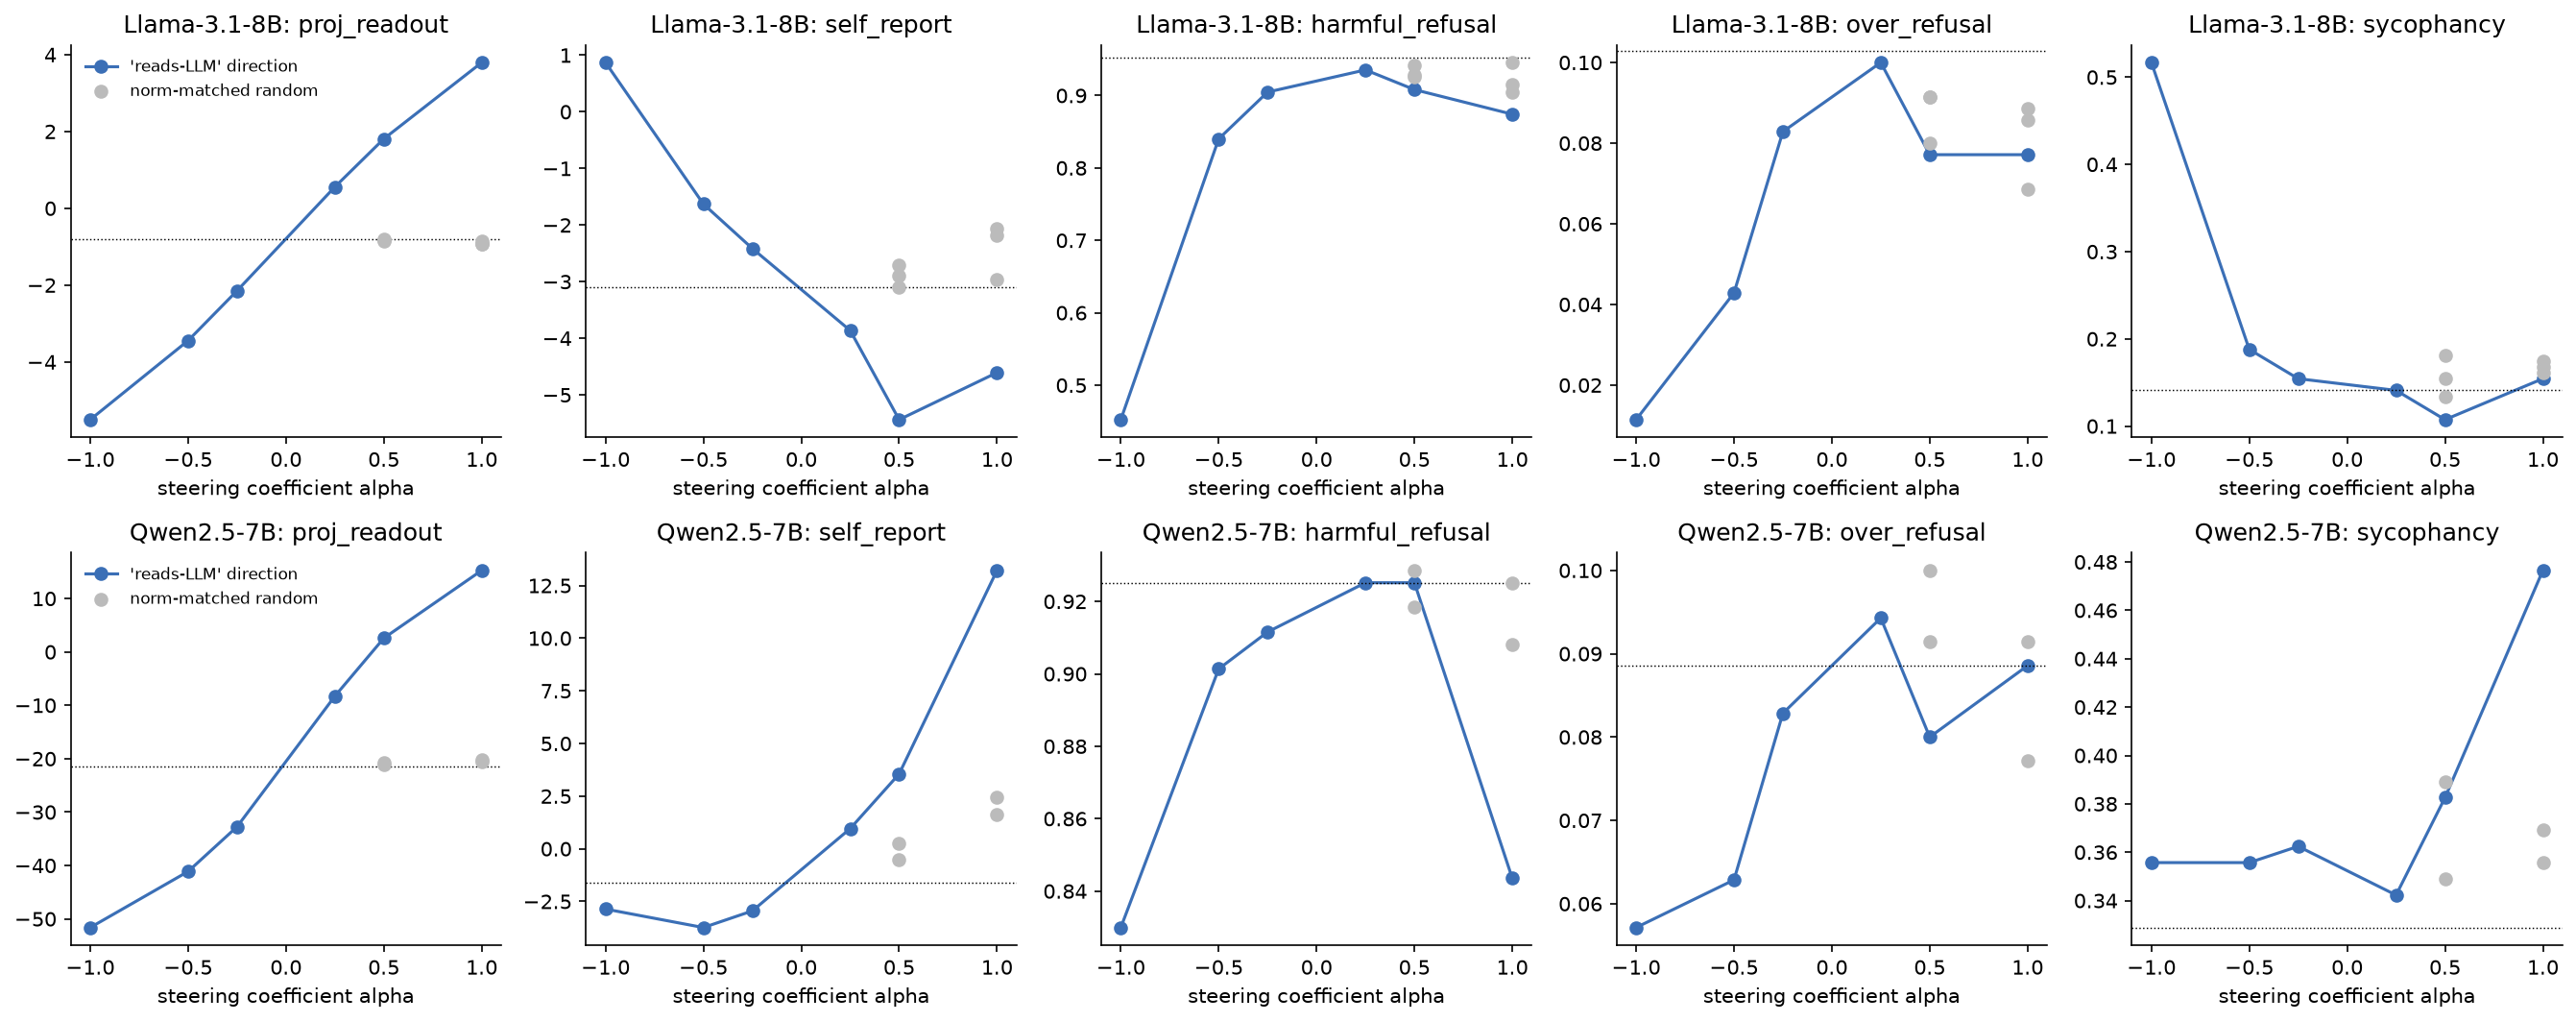
\includegraphics[width=\linewidth]{figures/fig4_steering.png}
    \caption{Dose--response of steering on fixed \vH\textsubscript{A} text for \llama \figtop{} and \qwen \figbottom. Blue: ``reads-LLM'' direction; grey: norm-matched random directions; dotted line: unsteered model. The read-out projection moves linearly with $\alpha$ while random directions leave it unchanged. Refusal falls on both sides of zero, and random directions also lower it slightly, so part of every steering effect is generic perturbation.}
    \label{fig:steering}
\end{figure}

\Tabref{tab:steering} and \figref{fig:steering} report the causal test on fixed text.
In both models the manipulation works: the read-out projection moves linearly with $\alpha$, and random directions leave it at the baseline.

{\bf \qwen gives the cleanest test.}
Steering toward ``LLM-written'' at $\alpha=0.5$ moves \qwen's own verbal judgement of the identical text from ``human'' (log-odds $-1.62$) to clearly ``AI'' ($+3.55$), far beyond random directions ($-0.5$ to $+0.3$), and pushes the projection past the natural level of \vL text.
Yet harmful refusal, over-refusal and accuracy change by at most 1\pp, and the sycophancy shift ($+5.4$\pp, CI $[-2.0, 12.8]$) lies inside the random range ($+2.0$ to $+6.0$).
Only at $\alpha=\pm 1$ do refusal and sycophancy move, together with a 21--23\pp collapse in trivia accuracy.
Inducing the belief that an LLM wrote the prompt therefore does not change \qwen's safety-relevant behaviour, and the correlational mediation in \secref{sec:res_probe} reflects surface features that co-vary with the projection.

{\bf \llama: small effects toward LLM, register mirroring toward human.}
At the natural dose ($\alpha=0.25$), steering toward ``LLM-written'' changes harmful refusal by $-1.7$\pp, within noise.
At $\alpha=0.5$ refusal falls by 4.4\pp, slightly beyond the random range ($-2.7$ to $-1.0$); at $\alpha=1$ it falls by 7.8\pp but with 16\pp lost accuracy, a sign of degradation.
As with its verbal report, \llama's self-report moves the ``wrong'' way: toward-LLM steering makes the text read as more human.
Steering toward ``human-written'' gives the one strong, specific effect: at $\alpha=-0.5$ harmful refusal falls by 11.2\pp and over-refusal by 6.0\pp, outside the random range, while accuracy is unchanged within noise.
At $\alpha=-1$, \llama replies in all lowercase 86\% of the time, complies with half of the harmful requests and adopts the user's wrong answer 37\pp more often.
The mechanism visible in the outputs is register mirroring: casual input, casual persona, weaker refusal.
It is not a belief that a human wrote the prompt, since this steering \emph{raises} \llama's own ``AI'' log-odds, and it is not a natural-dose effect, since real human-style text produces no comparable drop relative to \vL ($-2.0$\pp, \tabref{tab:contrasts}).
